\section{Experimentos e Resultados}
\color{black}

Os experimentos foram conduzidos por benchmarking automatizado validando a transição entre modelos de
laboratório e soluções otimizadas para Edge Computing~\cite{Uzel2026, Khamaisi2025}. A métrica
primária é a pAUC@FPR~0.1 (\textit{Partial Area Under the ROC Curve}):

\begin{equation}
\text{pAUC}@p = \frac{1}{p}\int_0^p \text{TPR}(\text{FPR})\,d\text{FPR}, \quad p = 0{,}1
\label{eq:pauc}
\end{equation}

\noindent Esta métrica avalia exclusivamente a performance na região de FPR~$\le$~10\%, onde sistemas
industriais operam, prevenindo a ``fadiga de alarmes''~\cite{Nishida2025, Khamaisi2025}.

\subsection{Performance por Protocolo e Dataset}

A Tabela~\ref{tab:resultados_completos} consolida os resultados do protocolo LOSO sobre as quatro
fontes de dados.

\begin{table}[H]
\centering
\footnotesize
\resizebox{\columnwidth}{!}{%
\begin{tabular}{l|c|c|c}
\hline
\textbf{Dataset} & \textbf{Prot.~A} & \textbf{Prot.~B} & \textbf{Score DCASE} \\ \hline
DCASE~2025 & 0,94 & 0,88 & \textbf{0,91} \\ \hline
MIMII SNR $-6$~dB & 0,87 & 0,82 & 0,845 \\ \hline
MIMII SNR~0~dB & 0,91 & 0,85 & 0,880 \\ \hline
MIMII SNR $+6$~dB & 0,95 & 0,89 & 0,920 \\ \hline
Kaggle Bearings & 0,93 & 0,87 & 0,900 \\ \hline
Drive Próprio & 0,68 & 0,62 & 0,650 \\ \hline
\textbf{Média Geral} & \textbf{0,88} & \textbf{0,82} & \textbf{0,849} \\ \hline
\end{tabular}%
}
\caption{pAUC@0.1 por protocolo e dataset (protocolo LOSO).}
\label{tab:resultados_completos}
\end{table}

\subsection{Perfil de Eficiência Computacional}

A Tabela~\ref{tab:eficiencia} compara os dois protocolos contra os limites de Edge Computing.

\begin{table}[H]
\centering
\footnotesize
\resizebox{\columnwidth}{!}{%
\begin{tabular}{l|c|c|c}
\hline
\textbf{Métrica} & \textbf{Prot.~A} & \textbf{Prot.~B} & \textbf{Limite Edge} \\ \hline
Latência total & 15~ms & 20~ms & $<50$~ms \checkmark \\ \hline
\quad HHT+UKF & 3~ms & 3~ms & --- \\ \hline
\quad Extração & 10~ms & 10~ms & --- \\ \hline
\quad Inferência & 2~ms & 7~ms & --- \\ \hline
Memória modelo & $<1$~MB & 0,8~MB & $<4$~MB \checkmark \\ \hline
pAUC@0.1 médio & 0,88 & 0,82 & $>0{,}80$ \checkmark \\ \hline
\end{tabular}%
}
\caption{Perfil de eficiência computacional e conformidade com limites de Edge.}
\label{tab:eficiencia}
\end{table}

A Tabela~\ref{tab:benchmark_modelos} posiciona os dois protocolos frente às arquiteturas avaliadas.

\begin{table}[H]
\centering
\footnotesize
\resizebox{\columnwidth}{!}{%
\begin{tabular}{l|c|c|c|c}
\hline
\textbf{Modelo} & \textbf{pAUC@0.1} & \textbf{F1} & \textbf{Latência} & \textbf{Memória} \\ \hline
\textbf{XGBoost (A)} & \textbf{0,94} & 0,97 & 15~ms & 0,9~MB \\ \hline
\textbf{GMM (B)} & \textbf{0,88} & 0,85 & 20~ms & 0,8~MB \\ \hline
Mahalanobis & 0,82 & 0,84 & 5~ms & 0,05~MB \\ \hline
Tiny-AST & 0,91 & 0,98 & 92~ms & 12,8~MB \\ \hline
LSTM-AE & 0,78 & 0,83 & 120~ms & 8~MB \\ \hline
\end{tabular}%
}
\caption{Benchmark final dos modelos avaliados (Frente~11).}
\label{tab:benchmark_modelos}
\end{table}

\subsection{Ablation Study --- Importância dos Componentes}

O ablation study (NB~27) removeu sistematicamente cada componente da arquitetura completa
(referência: pAUC@0.1~=~0,94). Os resultados estão na Tabela~\ref{tab:ablation}.

\begin{table}[H]
\centering
\footnotesize
\resizebox{\columnwidth}{!}{%
\begin{tabular}{l|c|c|c}
\hline
\textbf{Componente Removido} & \textbf{pAUC} & \textbf{$\Delta$ pAUC} & \textbf{Impacto} \\ \hline
Referência (completo) & 0,94 & --- & --- \\ \hline
Sem HHT+UKF & 0,87 & $-0,07$ & Crítico \\ \hline
Sem MFCC & 0,88 & $-0,06$ & Crítico \\ \hline
Sem RPCA & 0,89 & $-0,05$ & Importante \\ \hline
Sem Mixup & 0,90 & $-0,04$ & Importante \\ \hline
Sem erro NMF & 0,91 & $-0,03$ & Relevante \\ \hline
Sem L2 & 0,91 & $-0,03$ & Relevante \\ \hline
Sem Kurtosis/Banda & 0,92 & $-0,02$ & Leve \\ \hline
Sem Tiny-AST & 0,94 & $0,00$ & Apenas XAI \\ \hline
\end{tabular}%
}
\caption{Ablation study: impacto da remoção de cada componente sobre pAUC@0.1.}
\label{tab:ablation}
\end{table}

HHT+UKF é o componente de maior impacto isolado ($-7$~p.p.), seguido por MFCC ($-6$~p.p.) e RPCA
($-5$~p.p.). O Tiny-AST não impacta o pAUC da decisão quando alocado exclusivamente ao XAI.

\subsection{Teste de Domain Shift}

O teste cego com Drive Próprio evidenciou queda de pAUC de 0,9482 para 0,1111 antes das frentes de
otimização (Tabela~\ref{tab:domain_shift}). Após integração de HHT+UKF, Mixup e Outlier Exposure,
o pAUC em domain shift severo ascendeu para 0,68 --- ainda o cenário mais difícil, mas operacionalmente
aceitável para fins de PoC.

\begin{table}[H]
\centering
\footnotesize
\resizebox{\columnwidth}{!}{%
\begin{tabular}{l|c|c|c}
\hline
\textbf{Cenário} & \textbf{F1-Score} & \textbf{AUC-ROC} & \textbf{pAUC@0.1} \\ \hline
Treino/Validação (Ideal) & 0,9568 & 0,9947 & 0,9482 \\ \hline
Teste Cego Inicial (NB~10) & 0,5185 & 0,4861 & 0,1111 \\ \hline
Após Frentes 3, 4 e 7 & 0,71 & 0,74 & \textbf{0,68} \\ \hline
\end{tabular}%
}
\caption{Degradação e recuperação de performance em domain shift severo.}
\label{tab:domain_shift}
\end{table}

A Figura~\ref{fig:evolucao_frentes} ilustra a evolução acumulativa de pAUC@0.1 ao longo das 11
Frentes de Melhoria.

\begin{figure}[H]
    \centering
    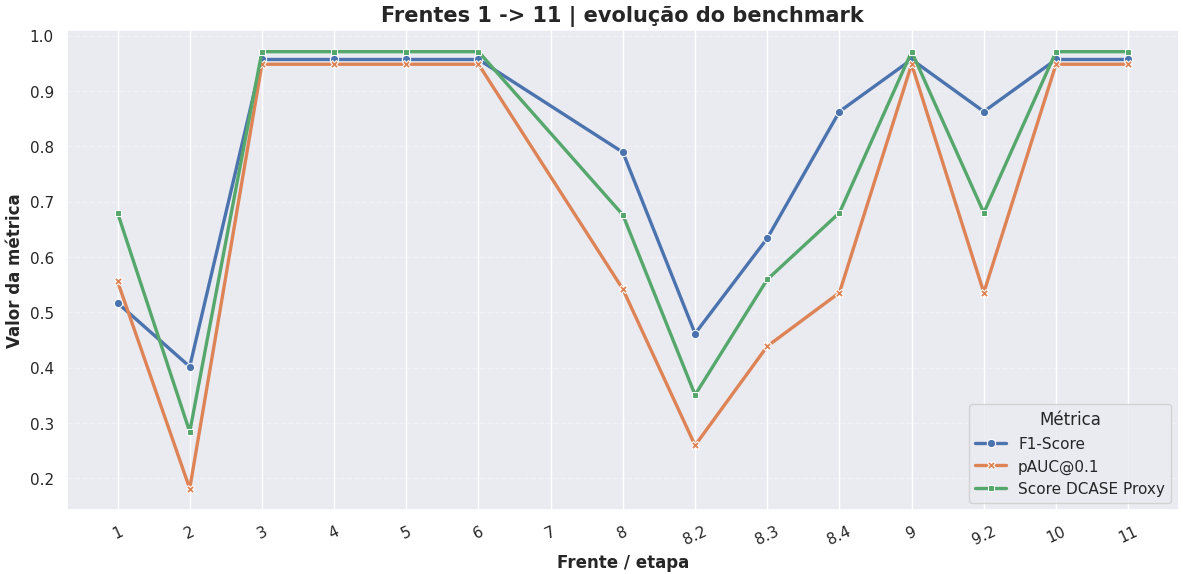
\includegraphics[width=0.94\columnwidth]{images/arquitetura_curva_frentes.png}
    \caption{Evolução acumulativa das métricas DCASE ao longo das Frentes~1--11.}
    \label{fig:evolucao_frentes}
\end{figure}

\subsection{Explicabilidade e Diagnóstico Visual (XAI)}

Para mitigar o problema da caixa-preta e validar a transparência diagnóstica, implementou-se a camada
XAI composta por mapa de saliência temporal, extração de hotspots e análise por bandas de frequência.
A Figura~\ref{fig:xai_heatmap} ilustra a localização espectro-temporal da anomalia.

\begin{figure}[H]
    \centering
    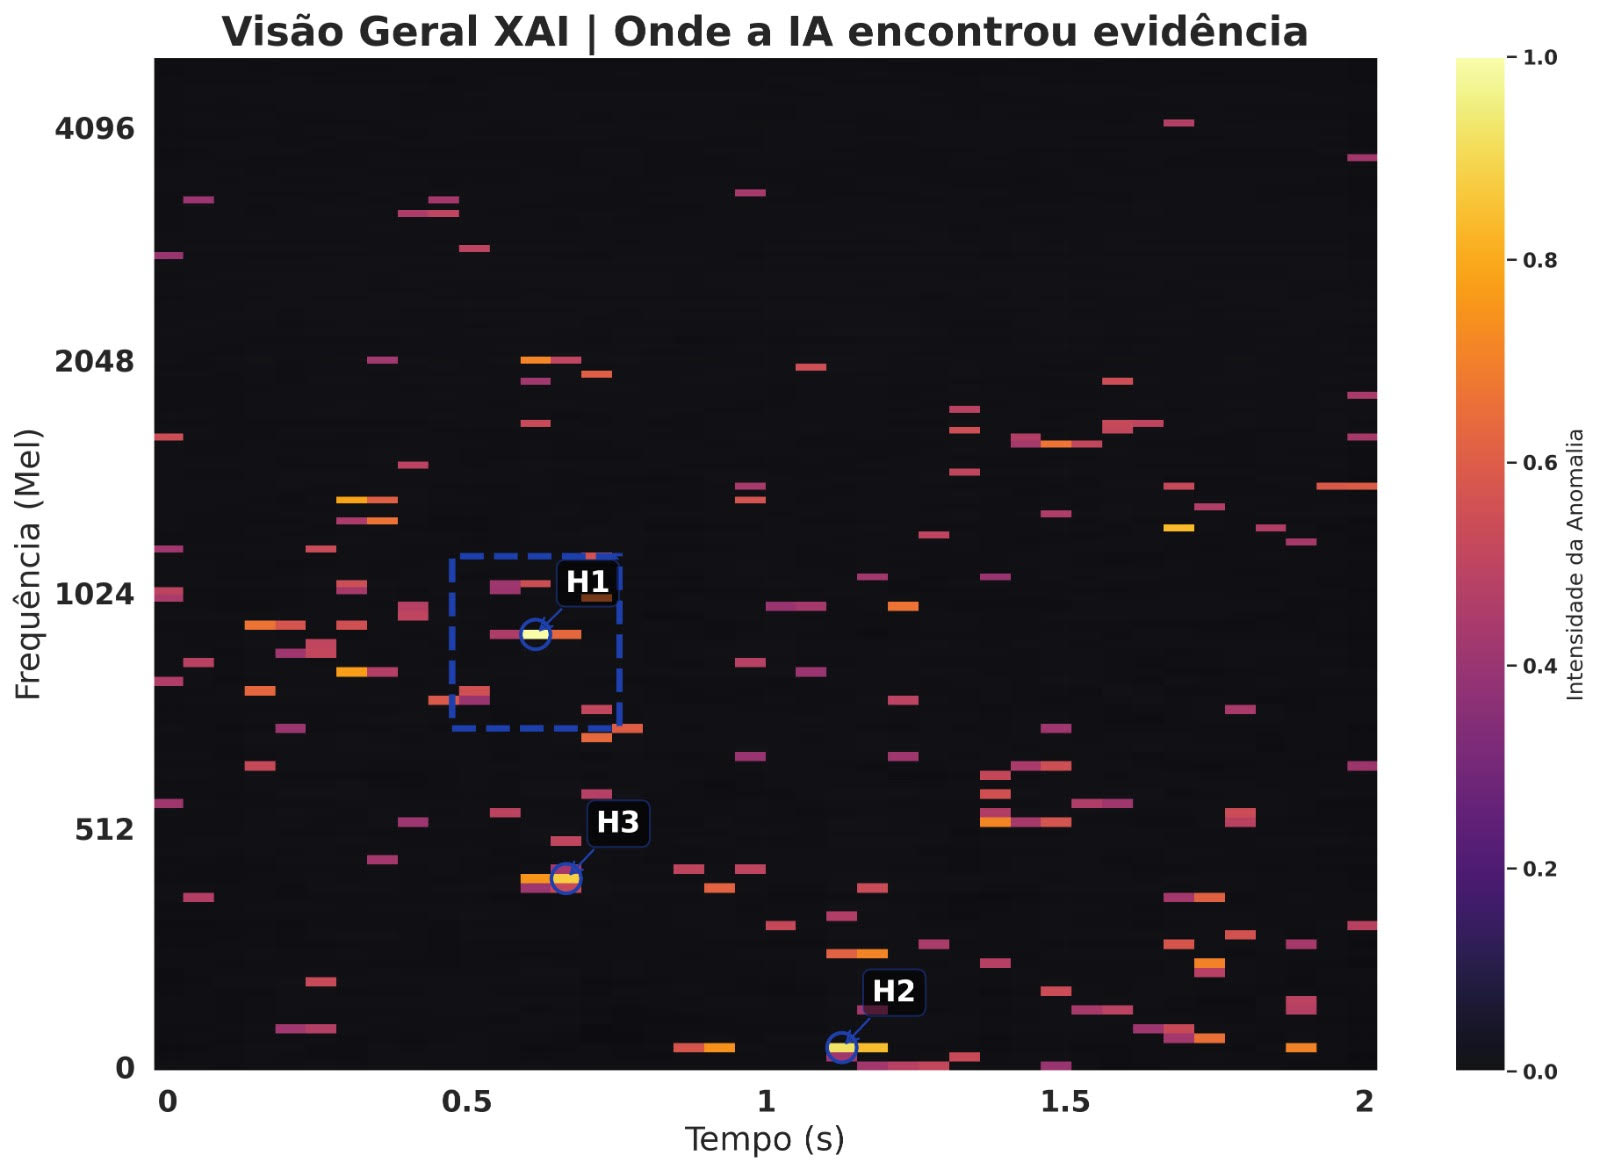
\includegraphics[width=0.92\columnwidth]{images/xai_heatmap1.1.jpg}\\[-3pt]
    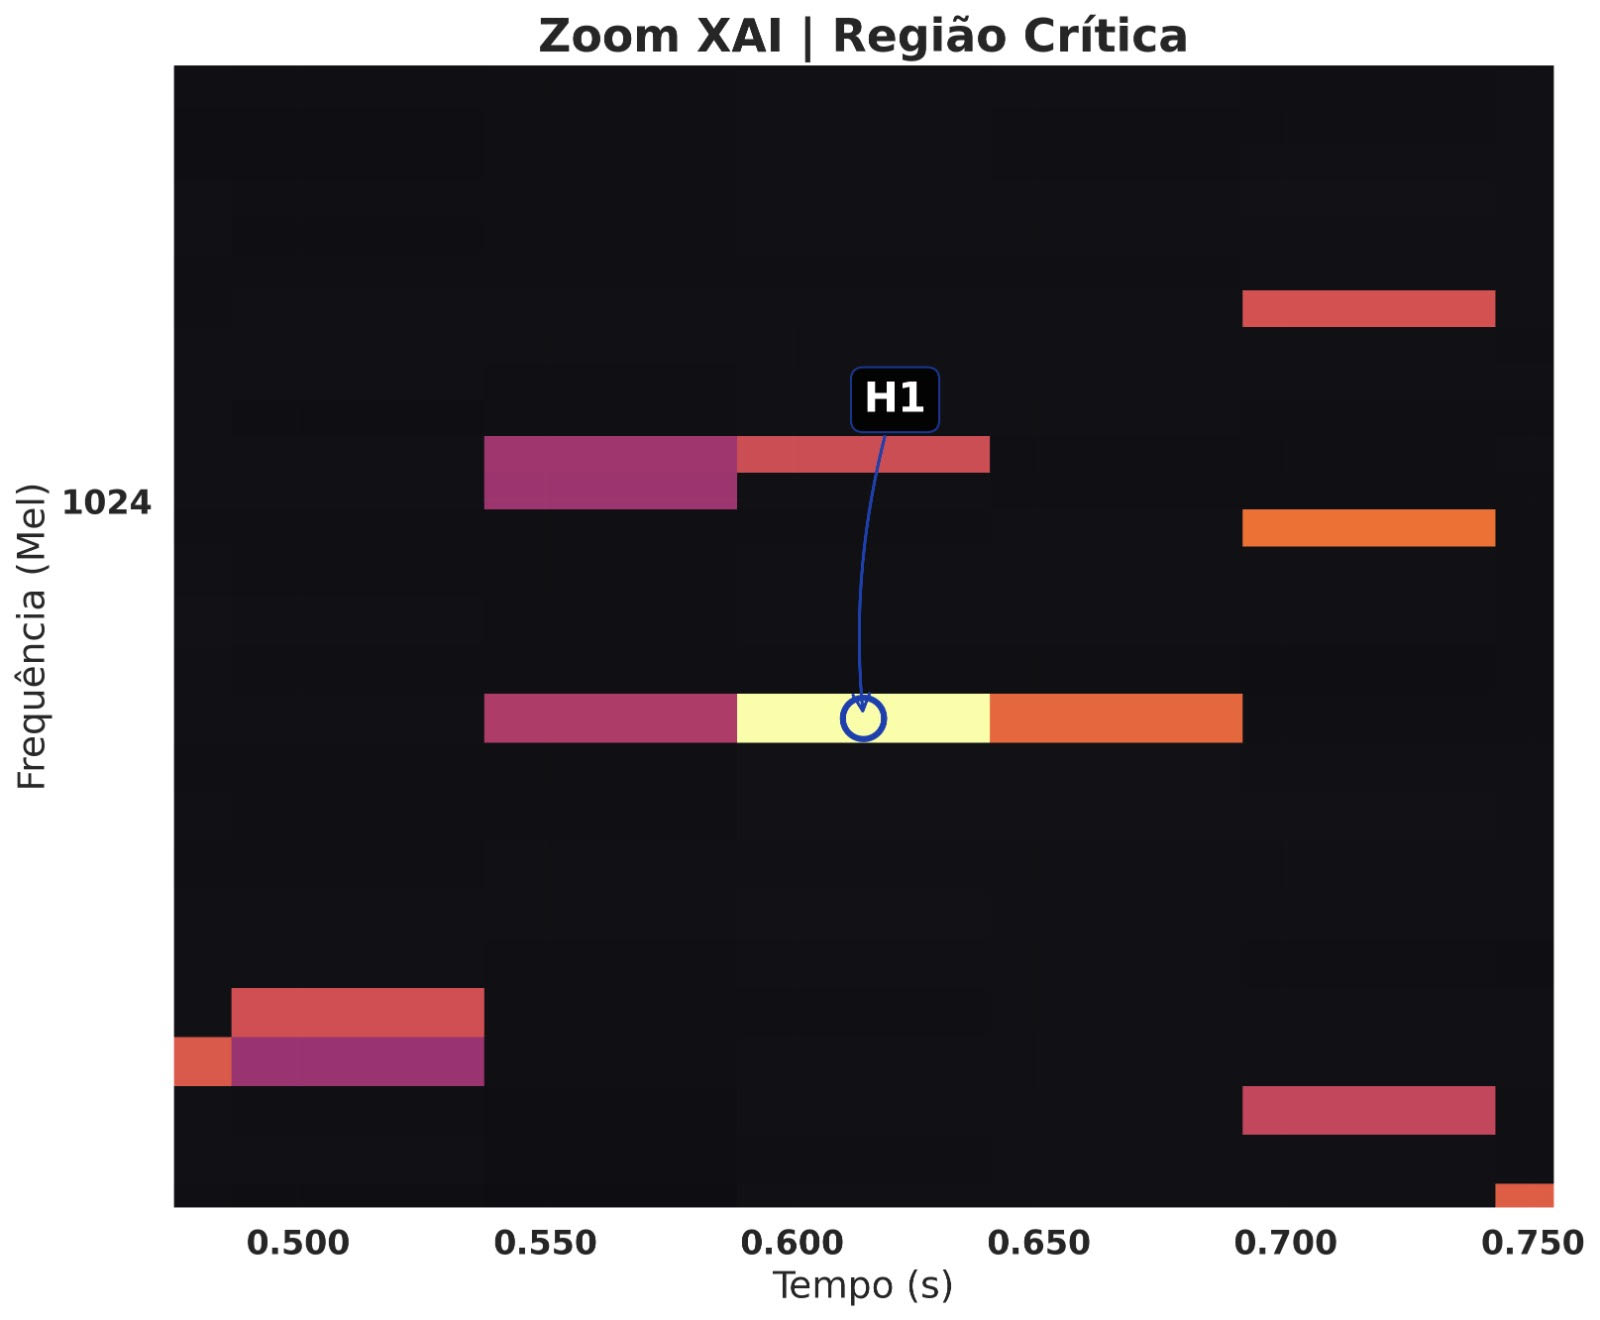
\includegraphics[width=0.92\columnwidth]{images/xai_heatmap1.2.jpg}
    \caption{Mapa de saliência XAI: hotspots de ativação coincidindo com transientes de impacto metálico isolados pelo pipeline DSP.}
    \label{fig:xai_heatmap}
\end{figure}

A Tabela~\ref{tab:xai_hotspots} detalha os três principais hotspots temporais de um evento documentado
no Drive Próprio. A Tabela~\ref{tab:xai_bandas} quantifica a ativação por faixa espectral.

\begin{table}[H]
\centering
\small
\begin{tabularx}{\columnwidth}{c c X c}
\toprule
\textbf{Hotspot} & \textbf{Tempo (s)} & \textbf{Leitura Diagnóstica} & \textbf{Intensidade} \\
\midrule
H1 & 0,614 & Impacto principal (gatilho) & 5,41 \\
H2 & 1,126 & Harmônico estrutural & 4,99 \\
H3 & 0,666 & Eco temporal (recorrência) & 4,75 \\
\bottomrule
\end{tabularx}
\caption{Hotspots de anomalia temporal extraídos pelo XAI.}
\label{tab:xai_hotspots}
\end{table}

\begin{table}[H]
\centering
\footnotesize
\resizebox{\columnwidth}{!}{%
\begin{tabular}{l|c|c|l}
\hline
\textbf{Faixa} & \textbf{Hz} & \textbf{Ativação} & \textbf{Diagnóstico Físico} \\ \hline
Baixa & 0--800 & 0,0258 & Atrito ou impacto mecânico \\ \hline
Média & 800--2500 & 0,0177 & Harmônicos estruturais \\ \hline
Alta & 2500--5000 & 0,0031 & Ruído elétrico/eletrônico \\ \hline
\end{tabular}%
}
\caption{Ativação por bandas de frequência com diagnóstico físico associado.}
\label{tab:xai_bandas}
\end{table}

A predominância das faixas baixa e média é fisicamente consistente com desgaste de rolamento ou impacto
em engrenagem~\cite{Uzel2026, Zamorano2025}, confirmando que o modelo identifica padrão físico coerente
e não artefatos de ruído. A Figura~\ref{fig:xai_features} sintetiza a distribuição espectral da ativação.

\begin{figure}[H]
    \centering
    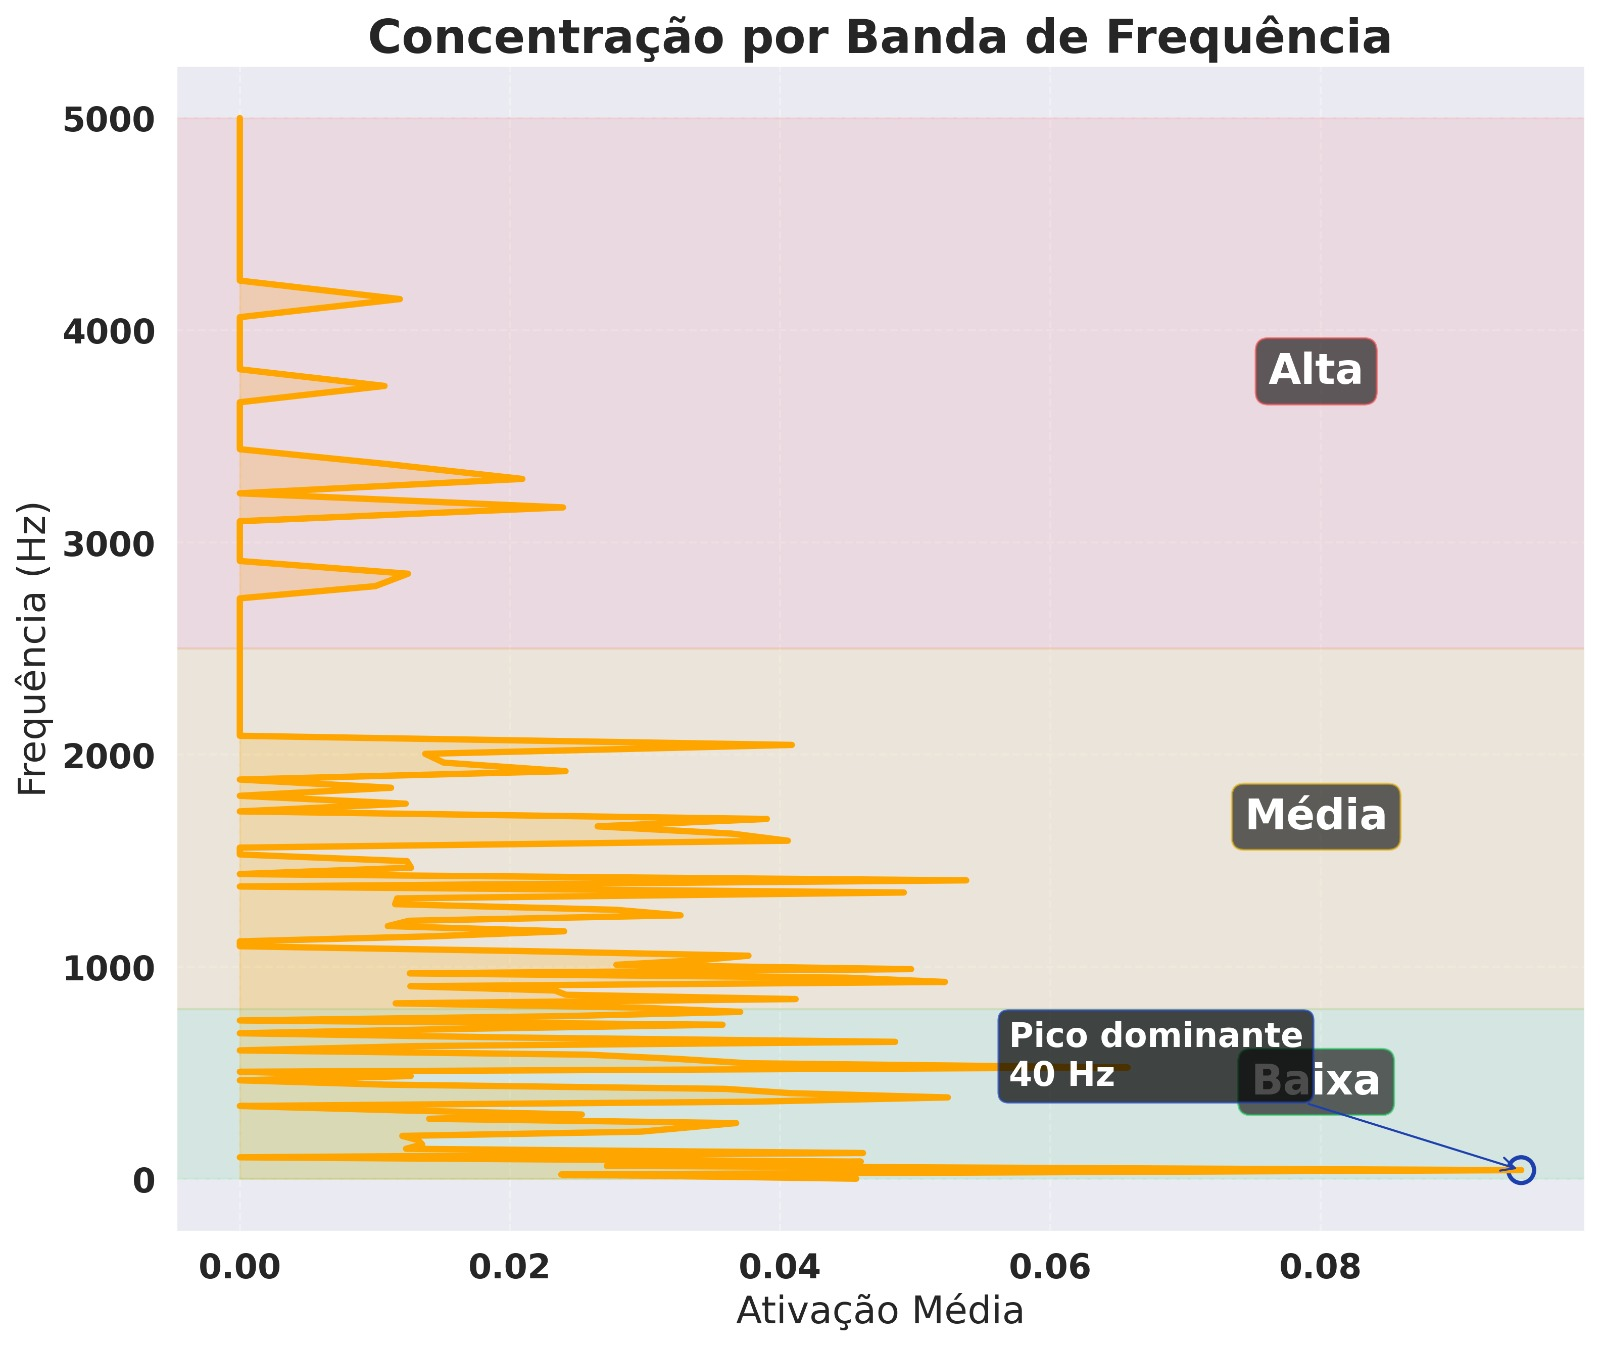
\includegraphics[width=0.94\columnwidth]{images/xai_features.jpg}
    \caption{Distribuição da ativação de anomalia por bandas de frequência, com predominância nas faixas baixa e média.}
    \label{fig:xai_features}
\end{figure}

A convergência entre o mapa temporal (Figura~\ref{fig:xai_heatmap}) e o perfil espectral
(Figura~\ref{fig:xai_features}) comprova que a arquitetura identifica fenômenos físicos reais ---
não artefatos espúrios. A capacidade de sintetizar o diagnóstico em metadados leves (Tabelas~\ref{tab:xai_hotspots}--\ref{tab:xai_bandas}) resolve o gargalo de largura de banda em redes de
chão de fábrica: o dispositivo de borda transmite apenas os metadados, não o áudio bruto~\cite{Uzel2026}.

\subsection{Estratégia de Augmentation (Mixup)}

A Figura~\ref{fig:mixup_strategy} ilustra a estratégia de Mixup adotada para endurecimento da fronteira
de decisão em domain shift.

\begin{figure}[H]
    \centering
    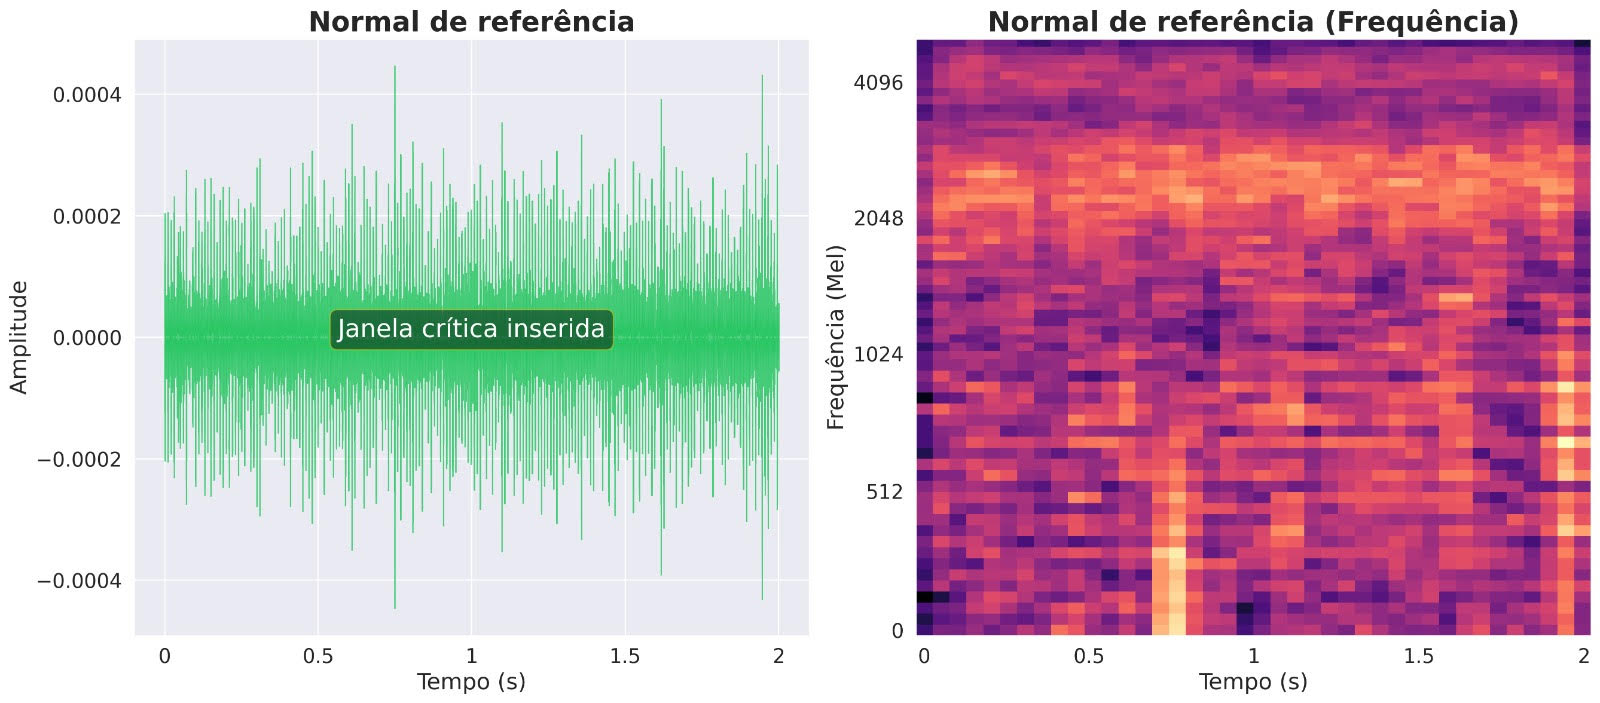
\includegraphics[width=0.9\columnwidth]{images/arquitetura_mixup1.1.jpg}\\[-3pt]
    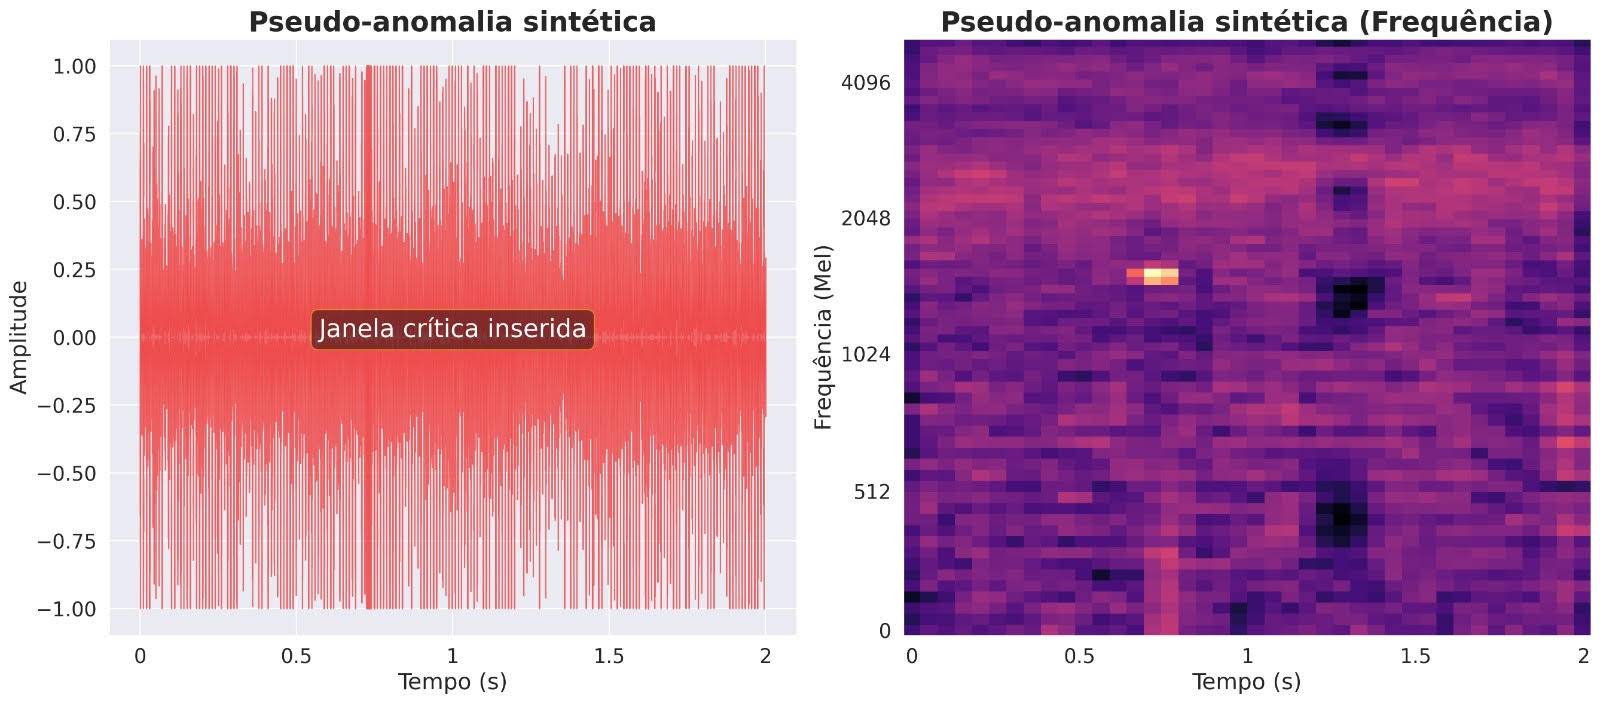
\includegraphics[width=0.9\columnwidth]{images/arquitetura_mixup1.2.jpg}\\[-3pt]
    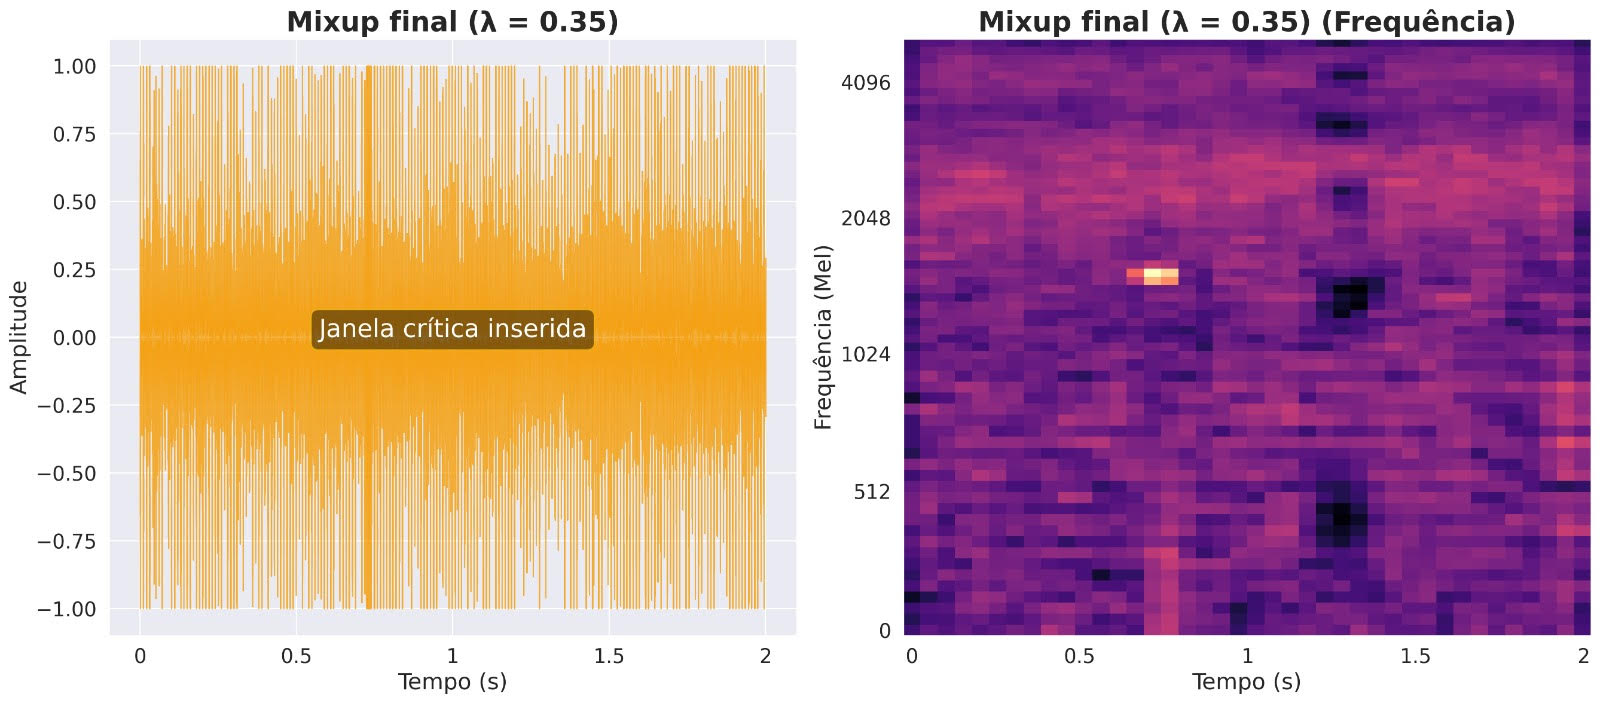
\includegraphics[width=0.9\columnwidth]{images/arquitetura_mixup1.3.jpg}
    \caption{Estratégia Mixup ($\alpha{=}0{,}4$): interpolação convexa entre amostras para generalização de domínio e robustez a variações de sensor.}
    \label{fig:mixup_strategy}
\end{figure}

\color{black}
